% new gaokao I q17 solution: pyramid P-ABCD with foot E on AC, F on PC
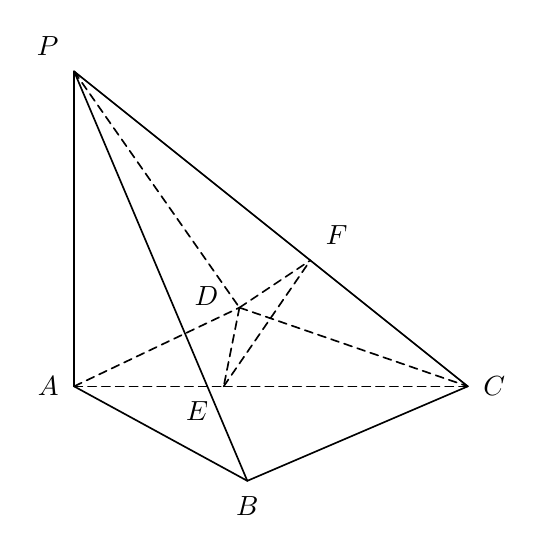
\begin{tikzpicture}[line width=.6pt, line join=round, line cap=round]
\coordinate (P) at (0.0000000000,5.2000000000);
\coordinate (A) at (0,1.2);
\coordinate (B) at (2.2,0);
\coordinate (C) at (5.0,1.2);
\coordinate (E) at (1.9,1.2);
\coordinate (D) at (2.1,2.2);
\coordinate (F) at (3.0000000000,2.8000000000);
% base ABCD (schematic projection, AC is diagonal)
\draw[densely dashed] (A) -- (E);
\draw[densely dashed] (E) -- (C);
\draw[solid] (A) -- (B);
\draw[solid] (B) -- (C);

\draw[densely dashed] (A) -- (D);
\draw[densely dashed] (D) -- (C);
\draw[densely dashed] (D) -- (E);
% lateral edges
\draw[solid] (P) -- (A);
\draw[solid] (P) -- (B);
\draw[solid] (P) -- (C);
\draw[densely dashed] (P) -- (D);

% auxiliary perpendiculars in solution
\draw[densely dashed] (D) -- (F);
\draw[densely dashed] (E) -- (F);
\node[above left=2pt] at (P) {$P$};
\node[left=2pt] at (A) {$A$};
\node[below=2pt] at (B) {$B$};
\node[right=2pt] at (C) {$C$};
\node[below left=2pt] at (E) {$E$};
\node[above left=2pt,xshift=-2pt,yshift=-5pt] at (D) {$D$};
\node[above right=2pt] at (F) {$F$};
\end{tikzpicture}
